%%%%%%%%%%%%%%%%%%%%%%%%%%%%%%%%%%%%%%%%%%%%%%%%%%%%%%%%%%%%%%%%
%
% Copyright (C) 2017-2019 Tactical Computing Laboratories, LLC
% All Rights Reserved
% contact@tactcomplabs.com
%
%%%%%%%%%%%%%%%%%%%%%%%%%%%%%%%%%%%%%%%%%%%%%%%%%%%%%%%%%%%%%%%%

%----------------------------------------------------------------------------------------
%	PACKAGES AND DOCUMENT CONFIGURATIONS
%----------------------------------------------------------------------------------------

\documentclass{article}

\usepackage[margin=1.0in]{geometry}
\usepackage[version=3]{mhchem} % Package for chemical equation typesetting
\usepackage{siunitx} % Provides the \SI{}{} and \si{} command for typesetting SI units
\usepackage{graphicx} % Required for the inclusion of images
%\usepackage{natbib} % Required to change bibliography style to APA
\usepackage{amsmath} % Required for some math elements 
\usepackage[utf8]{inputenc}
\usepackage[english]{babel}
\usepackage[parfill]{parskip}
\usepackage{array}
\usepackage{algorithm}
\usepackage{algcompatible}
\usepackage{listings}
\usepackage{xcolor}
\usepackage{courier} % for \texttt{}
\usepackage{dirtree}
\usepackage{multirow}
\usepackage{draftwatermark} % required for watermarks
\usepackage{vhistory}
\RequirePackage{epstopdf}
\RequirePackage{tabularx}
\RequirePackage{xstring}
\RequirePackage{hyperref}
\RequirePackage{fancyhdr}

%-- setup paragraphs and margins
\setlength{\parindent}{1em}
\setlength{\parskip}{1em}

\SetWatermarkText{DRAFT}
\SetWatermarkScale{5}

%-- code listing setup
\lstdefinestyle{base}{
  language=C++,
  numbers=left,
  stepnumber=1,
  emptylines=1,
  breaklines=true,
  basicstyle=\ttfamily\color{black},
  moredelim=**[is][\color{red}]{@}{@},
}

%-- setup hyperlinks
\hypersetup{
  colorlinks=true,
  linktoc=all,
  linkcolor=black,
  citecolor=black,
  urlcolor=black
}
%--

\setlength\parindent{0pt} % Removes all indentation from paragraphs

\renewcommand{\labelenumi}{\alph{enumi}.} % Make numbering in the enumerate environment by letter rather than number (e.g. section 6)

%\usepackage{times} % Uncomment to use the Times New Roman font
%----------------------------------------------------------------------------------------
%	DOCUMENT LAYOUT INFORMATION
%----------------------------------------------------------------------------------------
\pagestyle{fancy}
\lhead{}
\chead{\textbf{StoneCutter Language Spec v.0.1}}  % -- classification
\rhead{}
\lfoot{} %-- format: TR YYYY-RRR-V.V; y = year; r = report; v = version
\cfoot{\textbf{StoneCutter Language Spec v.0.1}}  % -- classification
\rfoot{\thepage}      % -- page number

%----------------------------------------------------------------------------------------
%	DOCUMENT INFORMATION
%----------------------------------------------------------------------------------------

\title{StoneCutter Language\\Specification} % Title

\author{Tactical Computing Laboratories, LLC} % Author name

\date{} % Date for the report

\begin{document}

%-- begin TCL logo
\begin{figure}
\begin{center}
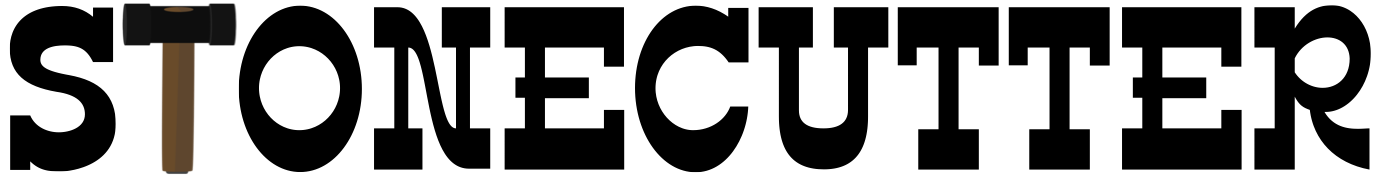
\includegraphics[width=5in]{figures/stonecutter.png} % Include the logo
\end{center}
\end{figure}
%-- end TCL logo

\maketitle % Insert the title, author and date
\thispagestyle{fancy} %-- force the fancyhdr

\begin{center}
\begin{tabular}{l r}
Date: & January 22, 2019 \\ % Date the experiment was performed
Revision: & 0.1 \\         % revision number
Authors: & Tactical Computing Labs\\ % Author names
& contact@tactcomplabs.com\\
\end{tabular}
\end{center}

% If you wish to include an abstract, uncomment the lines below
% \begin{abstract}
% Abstract text
% \end{abstract}

%----------------------------------------------------------------------------------------
%       TOC
%----------------------------------------------------------------------------------------

\clearpage
\tableofcontents
\clearpage

%----------------------------------------------------------------------------------------
%       List of Document Elements
%----------------------------------------------------------------------------------------

\clearpage
\listoffigures
\lstlistoflistings
\listoftables
%\listofalgorithms
\clearpage

%----------------------------------------------------------------------------------------
%       Changelog
%----------------------------------------------------------------------------------------

\clearpage
\begin{versionhistory}
  \vhEntry{0.1}{01.22.2018}{JLeidel}{Initial public release}
\end{versionhistory}
\clearpage

%----------------------------------------------------------------------------------------
%	SECTION 1
%----------------------------------------------------------------------------------------
\clearpage
\section{Overview}

The StoneCutter language is utilized to develop the implementation of a 
single instruction within the System Architect design workflow.  The StoneCutter 
language abstracts a large portion of traditional high level design languages such 
that the user may focus on the implementation details of a single instruction rather 
than the connectivity to the remainder of the infrastructure.  The core features of 
the StoneCutter language infrastructure are noted as follows: 

\begin{itemize}
\item \textbf{Compiled Language}: Unlike other HDL approaches, the StoneCutter language 
is, in fact, compiled.  The core StoneCutter compiler infrastructure makes use of the LLVM 
compiler infrastructure for lexing, parsing, optimization and code generation.  As a result, we have 
the ability to initiate traditional optimizing compiler passes, syntax tests and lexical analysis as 
other compiled languages.  Further, we have the ability to craft tooling that integrates with the StoneCutter 
language in the same manner as traditional compiled languages.  

\item \textbf{Integration with CoreGen IR}: The StoneCutter language and associated tooling is architected 
in a manner that permits integration with the CoreGen intermediate representation (IR)~\cite{IRSpec}.  This 
is done in two ways.  First, users have the ability to write StoneCutter instruction definitions inline within the 
CoreGen IR.  These \texttt{Impl} definitions are directly embedded within the overarching design.  Second, 
the CoreGen IR can be utilized to verify the I/O architecture and instruction format for each StoneCutter 
instruction definition.  This ensures that the prescribed instruction format in the CoreGen design is \textit{verified} 
to be functionally correct prior to utilizing downstream synthesis tools.      

\item \textbf{C-Like Syntax}: Unlike other HDL approaches, the StoneCutter language utilizes a familiar 
syntactical structure that is designed to mimic traditional C procedural methods.  Each instruction definition 
is contained within an effective function body with incoming arguments (registers).  Arithmetic, boolean operations, 
conditional operations and loop structures all mimic traditional procedural C syntax.  In this manner, the learning 
curve required to be productive with StoneCutter is minimized.  

\item \textbf{Support for Intrinsics}: Much in the same manner as traditional procedural languages such as C, 
StoneCutter has support for inline intrinsic operations.  Intrinsic operations are designed to support optimized 
circuits for pathological operations such as sign/zero extension, multi-input operations (majority vote, etc) and 
special arithmetic operations.  As the StoneCutter language continues to develop, we plan to augment the list 
of supported intrinsics.  

\end{itemize}


The remainder of this language specification is organized as follows.  Section~\ref{sec:StoneCutterLanguage} 
introduces the StoneCutter language and the associated syntax.  Section~\ref{sec:IntrinsicFunctions} provides 
details associated with each of the currently supported intrinsics.  Section~\ref{sec:AppendixA} provides 
a sample set of StoneCutter instruction definitions.  Section~\ref{sec:AppendixB} provides a consolidated list of StoneCutter 
intrinsics.  

 
%----------------------------------------------------------------------------------------
%	SECTION 2
%----------------------------------------------------------------------------------------
\clearpage
\section{StoneCutter Language}
\label{sec:StoneCutterLanguage}

\subsection{Overview}
\label{sec:LangOverview}

As mentioned above, the StoneCutter language is designed to take instruction definitions in a procedural syntax, 
optimize the instruction body and output each instruction in Chisel HDL.  As shown in Figure~\ref{fig:SCArch}, input 
files or buffers are parsed into an appropriate AST.  Instruction intrinsics are recognized and annotated in the AST.  Further, 
register classes and registers are identified and marked as special globals.  The AST is then translated to standard 
LLVM intermediate representation (IR).  The tools utilize standard LLVM optimization passes to optimize the instruction IR.  
The tools then execute a series of StoneCutter-specific IR passes against the optimized LLVM IR in order to ensure that the 
instruction design is correct per the prescribed instruction format(s).  Once verified as correct, the instruction intrinsics are expanded inline and the 
tools generate Chisel HDL.

\begin{figure}[h]
\begin{center}
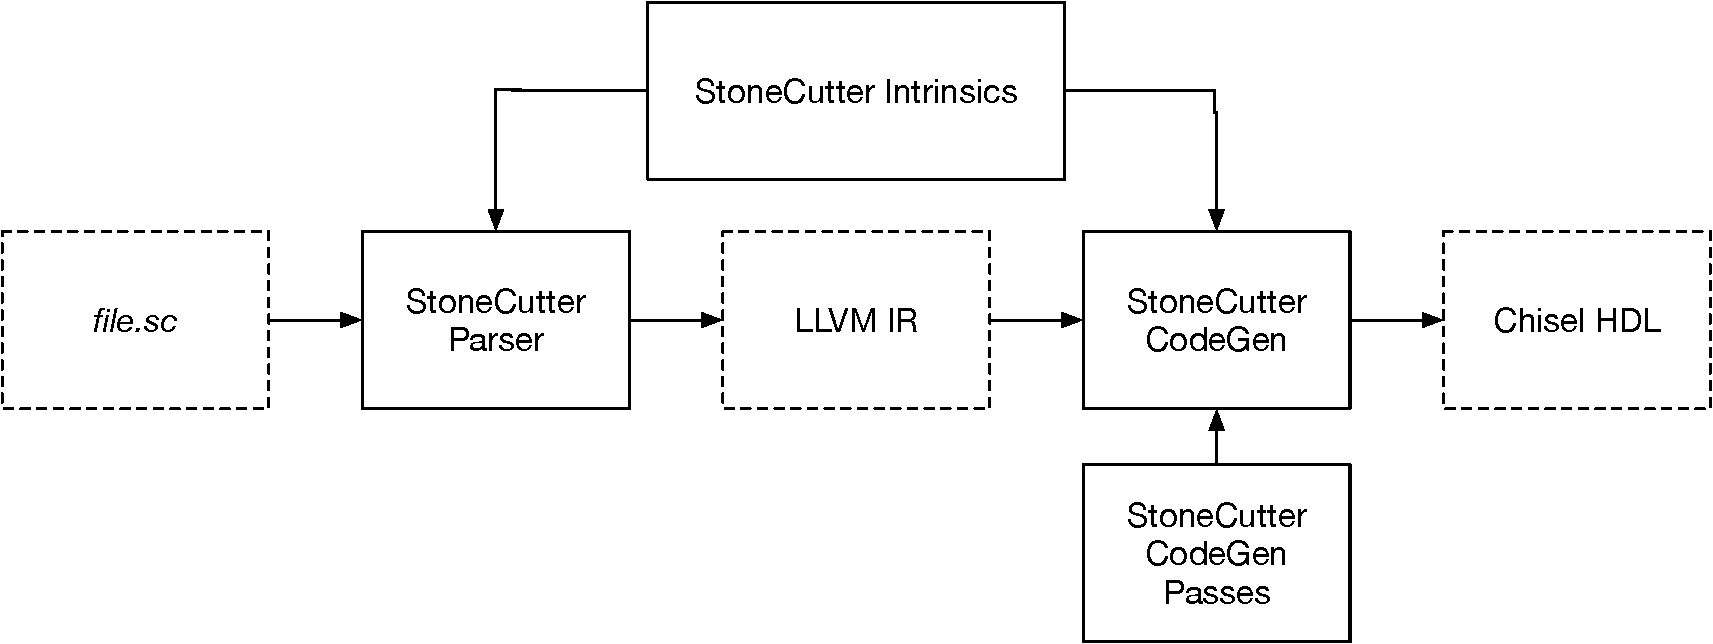
\includegraphics[width=\textwidth]{figures/scarch.pdf}
\vspace*{8pt}
\caption{StoneCutter Architecture}
\label{fig:SCArch}
\end{center}
\end{figure}

Each StoneCutter input file is constructed is a specific, prescribed manner.  The organization of the data members and 
the instruction definitions is done so specifically to elicit global and local hardware state within and across individual instructions.  
We find a sample of the StoneCutter file layout in Listing~\ref{lis:scoverview}.  
StoneCutter input files begin with an optional comment block describing the contents of the file.  Next, the individual register 
classes are defining for use by the instructions.  These register classes should match the register class definitions in name and 
layout found in the respective CoreGen design input.  Further information regarding the definition of register classes can 
be found in Section~\ref{sec:RegClassDef}.  The next portion of the file includes the actual instruction definitions.  Each 
instruction definition is comprised of a \textit{function}-like structure denoted with a \texttt{def} keyword.  Each instruction 
takes some number of instruction arguments (I/O's) and contains private variables and arithmetic logic.  Notice how 
the variable definitions are made near the top of the instruction definition.  Much like the C language, this is required 
in StoneCutter in order to preemptively understand the scope of the temporary variables defined in the instruction.  
Sections~\ref{sec:InstructionPrototypes}-\ref{sec:LoopOperations} 
describe the rudimentary operations and the associated syntax that can be included in the instruction 
definition body.  

\clearpage
\vspace{0.125in}
\begin{lstlisting}[frame=single,style=base,caption={StoneCutter File Structure},captionpos=b,label={lis:scoverview}]
#
# Sample StoneCutter File Layout
#

# Instruction Formats
instformat FORMAT1( FIELDTYPE FIELD1, FIELDTYPE FIELD2, ... )

# Register Class Definitions
regclass CLASS1( DATATYPE REG1, DATATYPE REG2, ... )
regclass CLASS2( DATATYPE REG3( DATATYPE SUBREG1, DATATYPE SUBREG2 ) )

# Instruction Definitions
def INST1( INPUT1 INPUT2 INPUT3 ) {
	# Variable Definitions
	DATATYPE VAR1, VAR2, VAR3
	DATATYPE VAR4
	
	# Instruction Body
	VAR4 = INPUT2 + INPUT1
	VAR1 = INPUT1 << 1
	VAR2 = INPUT3 << 2
	VAR3 = INPUT1 + INPUT2
	INPUT1 = VAR3
}

def INST2( REG1 REG3 SUBREG1 ) {
	# Instruction Body
	REG1 = REG3 * SUBREG1
}
\end{lstlisting}

\subsection{Syntactical Notes}
\label{sec:SyntacticalNotes}

Prior to reading the remaining sections, we highly suggest users and readers 
understand the following syntactical notes.  Understanding these notes will significantly 
reduce the time required to become productive in StoneCutter.  

\begin{itemize}
\item \textbf{Semicolons}: Unlike the C language, StoneCutter does not require utilizing semicolons (\texttt{;}) 
to terminate an expression.  All raw expressions are in static single assignment (SSA) form.  This implies 
that each expression will be in the form of \texttt{TARGET = INPUT <OP> OUTPUT}.  The only exception 
to this rule is when intrinsics are utilized.  A call to an intrinsic function may be

\item \textbf{Complement Operations}: The StoneCutter language contains all the standard arithmetic, boolean 
and logical operations except complements.  The bitwise complement operator from C (\texttt{\~}) is not supported 
and the boolean complement operator from C (\texttt{!}) is not supported.  Complementing the result of a boolean 
operation and/or performing the bitwise complement of a variable or register must be performed using the \texttt{NOT} 
intrinsic.  See Section~\ref{sec:NOT} for more details.   
\end{itemize}

\clearpage
\subsection{Comments}
\label{sec:Comments}

Inline comments and comment text in StoneCutter must begin with the pound (\texttt{\#}) sign.  Comments 
may begin on new lines on inline with other code.  Examples of using comments are shown in Listing~\ref{lis:comments}.  

\vspace{0.125in}
\begin{lstlisting}[frame=single,style=base,caption={StoneCutter Comments},captionpos=b,label={lis:comments}]
# This is a stand alone comment
def inst0(RA RB RT) {   # this is an inline comment
	RT = RA + RB
}
\end{lstlisting}

\clearpage
\subsection{Datatypes}
\label{sec:Datatypes}

Much in the same manner as traditional programming models such as C and C++, StoneCutter 
supports a common set of datatypes for intermediate variables and registers.  However, unlike 
traditional programming models, hardware design languages are required to support datatypes 
in non-byte aligned types.  In order to provide more hardware-centric support, StoneCutter supports 
traditional data types as well as arbitrary width signed and unsigned integer types.  These types are 
documented in Table~\ref{tab:datatypes}. 

\begin{table}[h]
\begin{center}
\caption{StoneCutter Datatypes}
\vspace{0.125in}
\label{tab:datatypes}
\begin{tabular}{|c|c|l|}
\hline
\textbf{Type} & \textbf{Width (in bits)} & \textbf{Description}\\
\hline
\texttt{bool} & 1 & Boolean.  Analogous to unsigned 1 bit integer (\texttt{u1})\\
\hline
\texttt{u8} & 8 & Unsigned 8 bit integer. Analogous to \texttt{uint8\_t}\\
\hline
\texttt{u16} & 16 & Unsigned 16 bit integer. Analogous to \texttt{uint16\_t}\\
\hline
\texttt{u32} & 32 & Unsigned 32 bit integer. Analogous to \texttt{uint32\_t}\\
\hline
\texttt{u64} & 64 & Unsigned 64 bit integer. Analogous to \texttt{uint64\_t}\\
\hline
\texttt{s8} & 8 & Signed 8 bit integer. Analogous to \texttt{int8\_t}\\
\hline
\texttt{s16} & 16 & Signed 16 bit integer. Analogous to \texttt{int16\_t}\\
\hline
\texttt{s32} & 32 & Signed 32 bit integer. Analogous to \texttt{int32\_t}\\
\hline
\texttt{s64} & 64 & Signed 64 bit integer. Analogous to \texttt{int64\_t}\\
\hline
\texttt{float} & 32 & Single precision floating point\\
\hline
\texttt{double} & 64 & Double precision floating point\\
\hline
\texttt{uN} & N bits & Arbitrary unsigned integer of N bits\\
\hline
\texttt{sN} & N bits & Arbitrary signed integer of N bits\\
\hline
\end{tabular}
\end{center}
\end{table}

An example of defining arbitrary width integers is shown in Listing~\ref{lis:arbwidth}.  

\vspace{0.125in}
\begin{lstlisting}[frame=single,style=base,caption={Arbitrary Width Datatypes},captionpos=b,label={lis:arbwidth}]
#-- unsigned 7 bit integer "foo"
u7 foo

#-- unsigned 1024 integer "bar"
u1024 bar

#-- signed 37 integer "foobar"
s37 foobar
\end{lstlisting}

\clearpage
\subsection{Instruction Format Definitions}
\label{sec:InstFormatDef}

Instruction formats and their associated fields are special variables in the StoneCutter language.  Each defined 
instruction field must reside within a respective instruction format.  Instruction fields are marked in the IR with 
attributes in order to ensure that they are correctly associated with the correct instruction format.  Further, for each 
field that is denoted as a register field, the associated register class must also be specified in order to correctly 
link the register read datapath to the correct register file.  Each of the associated fields is annotated as a global 
variable such that is can be explicitly utilized in any instruction prototype or instruction body.  

\begin{table}[h]
\begin{center}
\caption{StoneCutter Instruction Format Field Types}
\vspace{0.125in}
\label{tab:instformatfields}
\begin{tabular}{|c|c|c|l|}
\hline
\textbf{Field} & \textbf{Mnemonic} & Read/Write Access & \textbf{Description}\\
\hline
\multirow{2}{*}{Instruction Encodings} & \texttt{enc} & Read-Only & Instruction encodings such as\\
												  & & & opcodes and function codes\\
\hline
\multirow{2}{*}{Immediate Values} & \texttt{imm} & Read-Only & Immediate values encoded in the\\
											      & & & instruction payload\\
\hline
\multirow{3}{*}{Register Indices} & \texttt{reg[REGCLASS]} & Read-Write & Register index encodings.\\
														& & & Must include the respective\\
														& & & REGCLASS\\
\hline
\end{tabular}
\end{center}
\end{table}

For each field in the instruction format, the respective field is designated with a field type and a field name.  There are 
three types of instruction field types.  First, instruction fields denoted as encoding fields are utilized to designate 
individual instruction encodings such as opcodes and function codes in RISC architectures.  When utilizing these fields 
in the implementation of an instruction, the value contained within the field is utilized.  For example, if an instruction 
defines a field \texttt{opc} that contains the values 0x0A hex, reading from this field will provide the exact value 0x0A hex.  
Second, immediate fields are immediate values encoded directly within the instruction payload.  Reading from immediate 
fields from within the instruction payload will read the literal immediate from the instruction payload.  Finally, register fields 
denote register indices that access a single register file.  Reading from this field directly will not deliver the index.  Rather, accessing 
a register field will read or write the value at the designated index of the target register file.    
For fields that are denoted as register class fields (\texttt{reg}), the associated register class (register file) must also be specified.  
We summarize the permissible instruction field types in Table~\ref{tab:instformatfields}.  Further, the syntax for the an entire instruction 
format block is shown in Listing~\ref{lis:instformat}.  Encoding and immediate fields are always marked as read-only.  Only 
register fields may be written to.  

\vspace{0.125in}
\begin{lstlisting}[frame=single,style=base,caption={Instruction Format Definition Syntax},captionpos=b,label={lis:instformat}]
instformat FName1( FIELDTYPE FIELD1, FIELDTYPE FIELD2, ... )
instformat FName2( reg[REGCLASS] FIELD1, ... )
\end{lstlisting}

We find an example instruction format definition for a simple RISC ISA with encodings for an opcode and function code 
as well as three register fields in Listing~\ref{lis:sampleinstformat}.  

\vspace{0.125in}
\begin{lstlisting}[frame=single,style=base,caption={Sample Instruction Format Definition},captionpos=b,label={lis:sampleinstformat}]
instformat RISC( enc opc, enc func, reg[GPR] RT, reg[GPR] RA, reg[GPR] RB )
\end{lstlisting}

\clearpage
\subsection{Register Class Definitions}
\label{sec:RegClassDef}

Register classes and their associated registers are special variables in the StoneCutter language.  Each defined register 
is must reside within its respective register class.  Registers are marked in the IR with attributes in order to ensure that 
they belong to the correct register class when being utilized in an instruction body.  Each register is also annotated as a global 
variable such that it can be explicitly utilized in any instruction definition body.

\vspace{0.125in}
\begin{lstlisting}[frame=single,style=base,caption={Register Class Definition Syntax},captionpos=b,label={lis:regclass}]
regclass RCName1( DATATYPE RegName1, DATATYPE RegName2, ... )
regclass RCName2( DATATYPE RegName( DATATYPE SubReg1, DATATYPE SubReg2 ) )
\end{lstlisting}

We find the syntax for defining register classes and their associated registers in Listing~\ref{lis:regclass}.  Each register 
class is definition is marked with a \texttt{regclass} keyword followed by the register class name.  Each of the registers 
defined within the register class are enclosed within parenthesis.  Within the parenthesis, each register definition must 
be preceded by its respective datatype (Section~\ref{sec:Datatypes}) and the register name.  Registers are separated 
by commas.  For registers that have subfields, we may also explicitly annotate these within the register definition.  For 
each register with subfields, the subfields are defined within parenthesis attached to the register definition 
(Line 2 in Listing~\ref{lis:regclass}).  Each subfield must also contain its respective datatype.  The combined number of bits for 
all subfields within a register definition must not exceed the total number of bits in that register.  

We find an example register class definition for a simple RISC ISA in Listing~\ref{lis:sampleregclass}.  

\vspace{0.125in}
\begin{lstlisting}[frame=single,style=base,caption={Sample Register Class Definition},captionpos=b,label={lis:sampleregclass}]
regclass GPR( u64 r0, u64 r1, u64 r2, u64 r3, u64 r4, u64 r5, u64 r6, 
		       u64 r7, u64 r8, u64 r9, u64 r10, u64 r11, u64 r12, 
		       u64 r13, u64 r14, u64 r15, u64 r16, u64 r17, u64 r18,
		       u64 r19, u64 r20, u64 r21, u64 r22, u64 r23, u64 r24, 
		       u64 r25, u64 r26, u64 r27, u64 r28, u64 r29, u64 r30,
		       r64 r31 )
regclass CTRL( u64 pc, u64 exc, u64 ne, u64 gt, u64 lt, u64 gte,
			 u64 lte, u64 sp, u64 fp, u64 rp )
\end{lstlisting}

\clearpage
\subsection{Instruction Prototypes}
\label{sec:InstructionPrototypes}

For each instruction defined in the StoneCutter syntax, we must construct 
an instruction prototype.  The instruction prototype is an important and powerful 
feature of the StoneCutter language.  The instruction prototype drives two major 
features in the downstream Chisel HDL produced by a compiled StoneCutter input.  
First, the prototype describes the attachment of the respective instruction implementation 
to the instruction crack logic generated by the CoreGen IR.  The instruction mnemonic 
utilized in the instruction definition must match that of the instruction mnemonic defined 
in the CoreGen IR.  In this manner, the combined StoneCutter and CoreGen IR infrastructure 
logic can match the instruction crack implementation and the instruction implementation (et al. ALU).  

Second, the instruction definition argument list defines the set of standard I/O ports utilized by the 
instruction.  Standard I/O ports are utilized to pipeline register read and write operations within an 
optimized pipeline.  While it is entirely permissible to directly address registers or register files 
from within an instruction definition that are not defined in the argument list, the eventual downstream 
instruction implementation may require additional register read/write operations that induce pipeline 
stalls.  Keep in mind that standard I/O ports such as the clock, register hazarding and stall signals 
are automatically instantiated.  

\vspace{0.125in}
\begin{lstlisting}[frame=single,style=base,caption={Instruction Prototype Format},captionpos=b,label={lis:instprototypeformat}]
def INSTNAME( ARG1 ARG2 ARG3 ... ) {
}
\end{lstlisting}

As mentioned above, the instruction prototype includes two main structures: the instruction 
name and the instruction arguments (Listing~\ref{lis:instprototypeformat}).  The instruction name must match the associated instruction 
name defined in the CoreGen IR.  The instruction name is case sensitive.  
See the CoreGen IR specification for more information~\ref{IRSpec}.  The instruction 
argument list contains a set of register or register class names that define the standard I/O functions 
for the optimized pipeline.  The instruction argument list must match the set of register or register file designators 
in the instruction format for the target instruction. 
  
Register arguments are interpreted literally.  In this manner, a register I/O is performed to the specific 
register index denoted by the target register.  Register class arguments are interpreted logically.  The register 
class arguments utilize the index specified in the assembled instruction payload to load or store from the respective 
register index in the target register file.  

We see an example of a series of instruction prototypes in Listing~\ref{lis:instprototype}.  We utilize the register class 
and register definitions from Section~\ref{sec:RegClassDef}.  We define three instructions, \texttt{add}, \texttt{move} 
and \texttt{inc}.  The \texttt{add} instruction prototype contains a single argument, \texttt{GPR}, that defines I/O ports 
to/from the GPR register class.  The \texttt{move} instruction utilizes both the \texttt{GPR} and the \texttt{CTRL} 
register classes.  Finally, the \texttt{inc} instruction utilizes the explicit \texttt{pc} register as well as the \texttt{GPR} 
register class.  Notice that the arguments within the prototype are \textbf{not} separated by commas.  Further, we see 
that the associated instruction definition body is contained within a set of brackets (\texttt{\{\}}).  

\clearpage
\vspace{0.125in}
\begin{lstlisting}[frame=single,style=base,caption={Instruction Prototype Format},captionpos=b,label={lis:instprototype}]
regclass GPR( u64 r0, u64 r1, u64 r2, u64 r3, u64 r4, u64 r5, u64 r6, 
		       u64 r7, u64 r8, u64 r9, u64 r10, u64 r11, u64 r12, 
		       u64 r13, u64 r14, u64 r15, u64 r16, u64 r17, u64 r18,
		       u64 r19, u64 r20, u64 r21, u64 r22, u64 r23, u64 r24, 
		       u64 r25, u64 r26, u64 r27, u64 r28, u64 r29, u64 r30,
		       r64 r31 )
regclass CTRL( u64 pc, u64 exc, u64 ne, u64 gt, u64 lt, u64 gte,
			 u64 lte, u64 sp, u64 fp, u64 rp )

# add operation			 
def add( GPR ){
}

# move between GPR and CTRL 
def move( GPR CTRL ){
}

# increment PC by GPR
def inc( pc GPR ){
}


\end{lstlisting}

\clearpage
\subsection{Variable Definitions}
\label{sec:Variable Definitions}

In addition to utilizing register classes and register fields as variables within 
an instruction definition, users may also specify local, temporary variables 
in the instruction definition body.  These values may be utilized as temporary 
storage for complex, multi-stage operations, loop counters and other intermediate 
state.  The StoneCutter compiler infrastructure will make every effort to minimize the overall 
hardware impact of these intermediate values to the size and timing of the target design.  As a result, 
these temporary values may be optimized out and/or reused by adjacent instructions 
in the generated downstream Chisel HDL.  

In the same manner as individual registers, variables are required to have a defined type.  
These types follow the same convention as defined in Section~\ref{sec:Datatypes}.  Variable 
names may not collide with existing instruction format fields or register names.  Much in the same 
manner as the C language, StoneCutter permits users to define multiple, independent variables 
using the same datatype.  The format of 
variable definitions is noted in Listing~\ref{lis:vardefs}.  We provide an example of a series of 
variable definitions in Listing~\ref{lis:samplevardefs}.  

\vspace{0.125in}
\begin{lstlisting}[frame=single,style=base,caption={Variable Definitions},captionpos=b,label={lis:vardefs}]
def INST( ... ){
  DATATYPE name1
  DATATYPE name2, name3, ...
}
\end{lstlisting}

\vspace{0.125in}
\begin{lstlisting}[frame=single,style=base,caption={Sample Variable Definitions},captionpos=b,label={lis:samplevardefs}]
instformat RISC( enc opc, enc func, reg[GPR] RT, reg[GPR] RA, reg[GPR] RB )

def add( RT RA RB ){
  u64 var1, var2
  if( RA == RB ){
    var1 = 5
    var2 = 6
  }else{
    var1 = 7
    var2 = 998
  }
  RT = var1 & var2
}
\end{lstlisting}

\clearpage
\subsection{Arithmetic Operations}
\label{sec:Arithmetic Operations}

\clearpage
\subsection{Conditional Operations}
\label{sec:ConditionalOperations}

\clearpage
\subsection{Loop Operations}
\label{sec:LoopOperations}

%----------------------------------------------------------------------------------------
%	SECTION 3
%----------------------------------------------------------------------------------------
\clearpage
\section{Intrinsic Functions}
\label{sec:IntrinsicFunctions}

\subsection{Overview}
\label{sec:IntrinsicOverview}

\subsection{Arithmetic Intrinsics}
\label{sec:ArithIntrinsics}

\subsubsection{CLZ}
\label{sec:CLZ}

\begin{table}[h]
\begin{center}
\caption{CLZ Intrinsic}
\vspace{0.125in}
\label{tab:CLZIntrinsic}
\begin{tabular}{|c|l|}
\hline
\textbf{Mnemonic} & \texttt{STORE(RA,RB)}\\
\hline
\textbf{Description} & foo\\
\hline
\multirow{2}{*}{\textbf{Arguments}} & RA: Contains the data to be stored\\
                          			     & RB: Contains the target address \\
\hline
\multirow{3}{*}{\textbf{Example}} & def INST(RA RB RT)\{\\
                          			  &   STORE(RA, RB)\\
                                                    & \}\\
\hline
\textbf{Return} & Nothing is returned\\                                                    
\hline
\end{tabular}
\end{center}
\end{table}

\clearpage
\subsubsection{COMPRESS}
\label{sec:COMPRESS}

\begin{table}[h]
\begin{center}
\caption{COMPRESS Intrinsic}
\vspace{0.125in}
\label{tab:COMPRESSIntrinsic}
\begin{tabular}{|c|l|}
\hline
\textbf{Mnemonic} & \texttt{STORE(RA,RB)}\\
\hline
\textbf{Description} & foo\\
\hline
\multirow{2}{*}{\textbf{Arguments}} & RA: Contains the data to be stored\\
                          			     & RB: Contains the target address \\
\hline
\multirow{3}{*}{\textbf{Example}} & def INST(RA RB RT)\{\\
                          			  &   STORE(RA, RB)\\
                                                    & \}\\
\hline
\textbf{Return} & Nothing is returned\\                                                    
\hline
\end{tabular}
\end{center}
\end{table}

\clearpage
\subsubsection{COMPRESSM}
\label{sec:COMPRESSM}

\begin{table}[h]
\begin{center}
\caption{COMPRESSM Intrinsic}
\vspace{0.125in}
\label{tab:COMPRESSMIntrinsic}
\begin{tabular}{|c|l|}
\hline
\textbf{Mnemonic} & \texttt{STORE(RA,RB)}\\
\hline
\textbf{Description} & foo\\
\hline
\multirow{2}{*}{\textbf{Arguments}} & RA: Contains the data to be stored\\
                          			     & RB: Contains the target address \\
\hline
\multirow{3}{*}{\textbf{Example}} & def INST(RA RB RT)\{\\
                          			  &   STORE(RA, RB)\\
                                                    & \}\\
\hline
\textbf{Return} & Nothing is returned\\                                                    
\hline
\end{tabular}
\end{center}
\end{table}

\clearpage
\subsubsection{CTZ}
\label{sec:CTZ}

\begin{table}[h]
\begin{center}
\caption{CTZ Intrinsic}
\vspace{0.125in}
\label{tab:CTZIntrinsic}
\begin{tabular}{|c|l|}
\hline
\textbf{Mnemonic} & \texttt{STORE(RA,RB)}\\
\hline
\textbf{Description} & foo\\
\hline
\multirow{2}{*}{\textbf{Arguments}} & RA: Contains the data to be stored\\
                          			     & RB: Contains the target address \\
\hline
\multirow{3}{*}{\textbf{Example}} & def INST(RA RB RT)\{\\
                          			  &   STORE(RA, RB)\\
                                                    & \}\\
\hline
\textbf{Return} & Nothing is returned\\                                                    
\hline
\end{tabular}
\end{center}
\end{table}

\clearpage
\subsubsection{DOZ}
\label{sec:DOZ}

\begin{table}[h]
\begin{center}
\caption{DOZ Intrinsic}
\vspace{0.125in}
\label{tab:DOZIntrinsic}
\begin{tabular}{|c|l|}
\hline
\textbf{Mnemonic} & \texttt{STORE(RA,RB)}\\
\hline
\textbf{Description} & foo\\
\hline
\multirow{2}{*}{\textbf{Arguments}} & RA: Contains the data to be stored\\
                          			     & RB: Contains the target address \\
\hline
\multirow{3}{*}{\textbf{Example}} & def INST(RA RB RT)\{\\
                          			  &   STORE(RA, RB)\\
                                                    & \}\\
\hline
\textbf{Return} & Nothing is returned\\                                                    
\hline
\end{tabular}
\end{center}
\end{table}

\clearpage
\subsubsection{EXTRACTS}
\label{sec:EXTRACTS}

\begin{table}[h]
\begin{center}
\caption{EXTRACTS Intrinsic}
\vspace{0.125in}
\label{tab:EXTRACTSIntrinsic}
\begin{tabular}{|c|l|}
\hline
\textbf{Mnemonic} & \texttt{STORE(RA,RB)}\\
\hline
\textbf{Description} & foo\\
\hline
\multirow{2}{*}{\textbf{Arguments}} & RA: Contains the data to be stored\\
                          			     & RB: Contains the target address \\
\hline
\multirow{3}{*}{\textbf{Example}} & def INST(RA RB RT)\{\\
                          			  &   STORE(RA, RB)\\
                                                    & \}\\
\hline
\textbf{Return} & Nothing is returned\\                                                    
\hline
\end{tabular}
\end{center}
\end{table}

\clearpage
\subsubsection{EXTRACTZ}
\label{sec:EXTRACTZ}

\begin{table}[h]
\begin{center}
\caption{EXTRACTZ Intrinsic}
\vspace{0.125in}
\label{tab:EXTRACTZIntrinsic}
\begin{tabular}{|c|l|}
\hline
\textbf{Mnemonic} & \texttt{STORE(RA,RB)}\\
\hline
\textbf{Description} & foo\\
\hline
\multirow{2}{*}{\textbf{Arguments}} & RA: Contains the data to be stored\\
                          			     & RB: Contains the target address \\
\hline
\multirow{3}{*}{\textbf{Example}} & def INST(RA RB RT)\{\\
                          			  &   STORE(RA, RB)\\
                                                    & \}\\
\hline
\textbf{Return} & Nothing is returned\\                                                    
\hline
\end{tabular}
\end{center}
\end{table}

\clearpage
\subsubsection{INSERTS}
\label{sec:INSERTS}

\begin{table}[h]
\begin{center}
\caption{INSERTS Intrinsic}
\vspace{0.125in}
\label{tab:INSERTSIntrinsic}
\begin{tabular}{|c|l|}
\hline
\textbf{Mnemonic} & \texttt{STORE(RA,RB)}\\
\hline
\textbf{Description} & foo\\
\hline
\multirow{2}{*}{\textbf{Arguments}} & RA: Contains the data to be stored\\
                          			     & RB: Contains the target address \\
\hline
\multirow{3}{*}{\textbf{Example}} & def INST(RA RB RT)\{\\
                          			  &   STORE(RA, RB)\\
                                                    & \}\\
\hline
\textbf{Return} & Nothing is returned\\                                                    
\hline
\end{tabular}
\end{center}
\end{table}

\clearpage
\subsubsection{INSERTZ}
\label{sec:INSERTZ}

\begin{table}[h]
\begin{center}
\caption{INSERTZ Intrinsic}
\vspace{0.125in}
\label{tab:INSERTZIntrinsic}
\begin{tabular}{|c|l|}
\hline
\textbf{Mnemonic} & \texttt{STORE(RA,RB)}\\
\hline
\textbf{Description} & foo\\
\hline
\multirow{2}{*}{\textbf{Arguments}} & RA: Contains the data to be stored\\
                          			     & RB: Contains the target address \\
\hline
\multirow{3}{*}{\textbf{Example}} & def INST(RA RB RT)\{\\
                          			  &   STORE(RA, RB)\\
                                                    & \}\\
\hline
\textbf{Return} & Nothing is returned\\                                                    
\hline
\end{tabular}
\end{center}
\end{table}

\clearpage
\subsubsection{MAJ}
\label{sec:MAJ}

\begin{table}[h]
\begin{center}
\caption{MAJ Intrinsic}
\vspace{0.125in}
\label{tab:MAJIntrinsic}
\begin{tabular}{|c|l|}
\hline
\textbf{Mnemonic} & \texttt{STORE(RA,RB)}\\
\hline
\textbf{Description} & foo\\
\hline
\multirow{2}{*}{\textbf{Arguments}} & RA: Contains the data to be stored\\
                          			     & RB: Contains the target address \\
\hline
\multirow{3}{*}{\textbf{Example}} & def INST(RA RB RT)\{\\
                          			  &   STORE(RA, RB)\\
                                                    & \}\\
\hline
\textbf{Return} & Nothing is returned\\                                                    
\hline
\end{tabular}
\end{center}
\end{table}

\clearpage
\subsubsection{MAX}
\label{sec:MAX}

\begin{table}[h]
\begin{center}
\caption{MAX Intrinsic}
\vspace{0.125in}
\label{tab:MAXIntrinsic}
\begin{tabular}{|c|l|}
\hline
\textbf{Mnemonic} & \texttt{STORE(RA,RB)}\\
\hline
\textbf{Description} & foo\\
\hline
\multirow{2}{*}{\textbf{Arguments}} & RA: Contains the data to be stored\\
                          			     & RB: Contains the target address \\
\hline
\multirow{3}{*}{\textbf{Example}} & def INST(RA RB RT)\{\\
                          			  &   STORE(RA, RB)\\
                                                    & \}\\
\hline
\textbf{Return} & Nothing is returned\\                                                    
\hline
\end{tabular}
\end{center}
\end{table}

\clearpage
\subsubsection{MERGE}
\label{sec:MERGE}

\begin{table}[h]
\begin{center}
\caption{MERGE Intrinsic}
\vspace{0.125in}
\label{tab:MERGEIntrinsic}
\begin{tabular}{|c|l|}
\hline
\textbf{Mnemonic} & \texttt{STORE(RA,RB)}\\
\hline
\textbf{Description} & foo\\
\hline
\multirow{2}{*}{\textbf{Arguments}} & RA: Contains the data to be stored\\
                          			     & RB: Contains the target address \\
\hline
\multirow{3}{*}{\textbf{Example}} & def INST(RA RB RT)\{\\
                          			  &   STORE(RA, RB)\\
                                                    & \}\\
\hline
\textbf{Return} & Nothing is returned\\                                                    
\hline
\end{tabular}
\end{center}
\end{table}

\clearpage
\subsubsection{MIN}
\label{sec:MIN}

\begin{table}[h]
\begin{center}
\caption{MIN Intrinsic}
\vspace{0.125in}
\label{tab:MINIntrinsic}
\begin{tabular}{|c|l|}
\hline
\textbf{Mnemonic} & \texttt{STORE(RA,RB)}\\
\hline
\textbf{Description} & foo\\
\hline
\multirow{2}{*}{\textbf{Arguments}} & RA: Contains the data to be stored\\
                          			     & RB: Contains the target address \\
\hline
\multirow{3}{*}{\textbf{Example}} & def INST(RA RB RT)\{\\
                          			  &   STORE(RA, RB)\\
                                                    & \}\\
\hline
\textbf{Return} & Nothing is returned\\                                                    
\hline
\end{tabular}
\end{center}
\end{table}

\clearpage
\subsubsection{NOT}
\label{sec:NOT}

\begin{table}[h]
\begin{center}
\caption{NOT Intrinsic}
\vspace{0.125in}
\label{tab:NOTIntrinsic}
\begin{tabular}{|c|l|}
\hline
\textbf{Mnemonic} & \texttt{STORE(RA,RB)}\\
\hline
\textbf{Description} & foo\\
\hline
\multirow{2}{*}{\textbf{Arguments}} & RA: Contains the data to be stored\\
                          			     & RB: Contains the target address \\
\hline
\multirow{3}{*}{\textbf{Example}} & def INST(RA RB RT)\{\\
                          			  &   STORE(RA, RB)\\
                                                    & \}\\
\hline
\textbf{Return} & Nothing is returned\\                                                    
\hline
\end{tabular}
\end{center}
\end{table}

\clearpage
\subsubsection{POPCOUNT}
\label{sec:POPCOUNT}

\begin{table}[h]
\begin{center}
\caption{POPCOUNT Intrinsic}
\vspace{0.125in}
\label{tab:POPCOUNTIntrinsic}
\begin{tabular}{|c|l|}
\hline
\textbf{Mnemonic} & \texttt{STORE(RA,RB)}\\
\hline
\textbf{Description} & foo\\
\hline
\multirow{2}{*}{\textbf{Arguments}} & RA: Contains the data to be stored\\
                          			     & RB: Contains the target address \\
\hline
\multirow{3}{*}{\textbf{Example}} & def INST(RA RB RT)\{\\
                          			  &   STORE(RA, RB)\\
                                                    & \}\\
\hline
\textbf{Return} & Nothing is returned\\                                                    
\hline
\end{tabular}
\end{center}
\end{table}

\clearpage
\subsubsection{REVERSE}
\label{sec:REVERSE}

\begin{table}[h]
\begin{center}
\caption{REVERSE Intrinsic}
\vspace{0.125in}
\label{tab:REVERSEIntrinsic}
\begin{tabular}{|c|l|}
\hline
\textbf{Mnemonic} & \texttt{STORE(RA,RB)}\\
\hline
\textbf{Description} & foo\\
\hline
\multirow{2}{*}{\textbf{Arguments}} & RA: Contains the data to be stored\\
                          			     & RB: Contains the target address \\
\hline
\multirow{3}{*}{\textbf{Example}} & def INST(RA RB RT)\{\\
                          			  &   STORE(RA, RB)\\
                                                    & \}\\
\hline
\textbf{Return} & Nothing is returned\\                                                    
\hline
\end{tabular}
\end{center}
\end{table}

\clearpage
\subsubsection{ROTL}
\label{sec:ROTL}

\begin{table}[h]
\begin{center}
\caption{ROTL Intrinsic}
\vspace{0.125in}
\label{tab:ROTLIntrinsic}
\begin{tabular}{|c|l|}
\hline
\textbf{Mnemonic} & \texttt{STORE(RA,RB)}\\
\hline
\textbf{Description} & foo\\
\hline
\multirow{2}{*}{\textbf{Arguments}} & RA: Contains the data to be stored\\
                          			     & RB: Contains the target address \\
\hline
\multirow{3}{*}{\textbf{Example}} & def INST(RA RB RT)\{\\
                          			  &   STORE(RA, RB)\\
                                                    & \}\\
\hline
\textbf{Return} & Nothing is returned\\                                                    
\hline
\end{tabular}
\end{center}
\end{table}

\clearpage
\subsubsection{ROTR}
\label{sec:ROTR}

\begin{table}[h]
\begin{center}
\caption{ROTR Intrinsic}
\vspace{0.125in}
\label{tab:ROTRIntrinsic}
\begin{tabular}{|c|l|}
\hline
\textbf{Mnemonic} & \texttt{STORE(RA,RB)}\\
\hline
\textbf{Description} & foo\\
\hline
\multirow{2}{*}{\textbf{Arguments}} & RA: Contains the data to be stored\\
                          			     & RB: Contains the target address \\
\hline
\multirow{3}{*}{\textbf{Example}} & def INST(RA RB RT)\{\\
                          			  &   STORE(RA, RB)\\
                                                    & \}\\
\hline
\textbf{Return} & Nothing is returned\\                                                    
\hline
\end{tabular}
\end{center}
\end{table}

\clearpage
\subsubsection{SEXT}
\label{sec:SEXT}

\begin{table}[h]
\begin{center}
\caption{SEXT Intrinsic}
\vspace{0.125in}
\label{tab:SEXTIntrinsic}
\begin{tabular}{|c|l|}
\hline
\textbf{Mnemonic} & \texttt{STORE(RA,RB)}\\
\hline
\textbf{Description} & foo\\
\hline
\multirow{2}{*}{\textbf{Arguments}} & RA: Contains the data to be stored\\
                          			     & RB: Contains the target address \\
\hline
\multirow{3}{*}{\textbf{Example}} & def INST(RA RB RT)\{\\
                          			  &   STORE(RA, RB)\\
                                                    & \}\\
\hline
\textbf{Return} & Nothing is returned\\                                                    
\hline
\end{tabular}
\end{center}
\end{table}

\clearpage
\subsubsection{ZEXT}
\label{sec:ZEXT}

\begin{table}[h]
\begin{center}
\caption{ZEXT Intrinsic}
\vspace{0.125in}
\label{tab:ZEXTIntrinsic}
\begin{tabular}{|c|l|}
\hline
\textbf{Mnemonic} & \texttt{ZEXT(RA,RB)}\\
\hline
\textbf{Description} & foo\\
\hline
\multirow{2}{*}{\textbf{Arguments}} & RA: Contains the data to be stored\\
                          			     & RB: Contains the target address \\
\hline
\multirow{3}{*}{\textbf{Example}} & def INST(RA RB RT)\{\\
                          			  &   STORE(RA, RB)\\
                                                    & \}\\
\hline
\textbf{Return} & Nothing is returned\\                                                    
\hline
\end{tabular}
\end{center}
\end{table}

\clearpage
\subsection{Memory Intrinsics}
\label{sec:MemIntrinsics}

\subsubsection{LOAD}
\label{sec:LOAD}

\begin{table}[h]
\begin{center}
\caption{LOAD Intrinsic}
\vspace{0.125in}
\label{tab:LOADIntrinsic}
\begin{tabular}{|c|l|}
\hline
\textbf{Mnemonic} & \texttt{LOAD(RA)}\\
\hline
\textbf{Description} & foo\\
\hline
\multirow{2}{*}{\textbf{Arguments}} & RA: Contains the target address \\
\hline
\multirow{3}{*}{\textbf{Example}} & def INST(RA RB RT)\{\\
                          			  &   RT = LOAD(RA)\\
                                                    & \}\\
\hline
\textbf{Return} & The data from the load operation\\                                                    
\hline
\end{tabular}
\end{center}
\end{table}

\clearpage
\subsubsection{STORE}
\label{sec:STORE}

\begin{table}[h]
\begin{center}
\caption{STORE Intrinsic}
\vspace{0.125in}
\label{tab:STOREIntrinsic}
\begin{tabular}{|c|l|}
\hline
\textbf{Mnemonic} & \texttt{STORE(RA,RB)}\\
\hline
\textbf{Description} & foo\\
\hline
\multirow{2}{*}{\textbf{Arguments}} & RA: Contains the data to be stored\\
                          			     & RB: Contains the target address \\
\hline
\multirow{3}{*}{\textbf{Example}} & def INST(RA RB RT)\{\\
                          			  &   STORE(RA, RB)\\
                                                    & \}\\
\hline
\textbf{Return} & Nothing is returned\\                                                    
\hline
\end{tabular}
\end{center}
\end{table}

\clearpage
\subsubsection{LOADELEM}
\label{sec:LOADELEM}

\begin{table}[h]
\begin{center}
\caption{LOADELEM Intrinsic}
\vspace{0.125in}
\label{tab:LOADELEMIntrinsic}
\begin{tabular}{|c|l|}
\hline
\textbf{Mnemonic} & \texttt{LOADELEM(RA,RB)}\\
\hline
\textbf{Description} & foo\\
\hline
\multirow{2}{*}{\textbf{Arguments}} & RA: Contains the target address\\
                          			     & RB: Contains the size of the element \\
\hline
\multirow{3}{*}{\textbf{Example}} & def INST(RA RB RT)\{\\
                          			  &   RT = LOADELEM(RA, RB)\\
                                                    & \}\\
\hline
\textbf{Return} & The data from the load operation\\                                                    
\hline
\end{tabular}
\end{center}
\end{table}

\clearpage
\subsubsection{STOREELEM}
\label{sec:STOREELEM}

\begin{table}[h]
\begin{center}
\caption{STOREELEM Intrinsic}
\vspace{0.125in}
\label{tab:STOREELEMIntrinsic}
\begin{tabular}{|c|l|}
\hline
\textbf{Mnemonic} & \texttt{STOREELEM(RA,RB,RC)}\\
\hline
\textbf{Description} & foo\\
\hline
\multirow{3}{*}{\textbf{Arguments}} & RA: Contains the data to be stored\\
                          			     & RB: Contains the target address \\
			     			     & RC: Contains the size of the element \\
\hline
\multirow{3}{*}{\textbf{Example}} & def INST(RA RB RC RT)\{\\
                          			  &   STOREELEM(RA, RB, RC)\\
                                                    & \}\\
\hline
\textbf{Return} & Nothing is returned\\                                                    
\hline
\end{tabular}
\end{center}
\end{table}

%----------------------------------------------------------------------------------------
%	SECTION: Appendix A: Sample IR
%----------------------------------------------------------------------------------------
\clearpage
\section{Appendix A: Sample StoneCutter Implementation}
\label{sec:AppendixA}

\vspace{0.125in}
\lstinputlisting[frame=single,style=base,caption={Sample StoneCutter},captionpos=b,label={lis:samplescfile}]{SAMPLE.sc}

%----------------------------------------------------------------------------------------
%	SECTION: Appendix B: Intrinsic Operation Table
%----------------------------------------------------------------------------------------
\clearpage
\section{Appendix B: Intrinsic Function Table}
\label{sec:AppendixB}

\begin{table}[h]
\begin{center}
\caption{StoneCutter Intrinsics}
\vspace{0.125in}
\label{tab:scintrins}
\begin{tabular}{|c|c|c|l|l}
\hline
\textbf{Intrinsic} & \textbf{Inputs} & \textbf{Outputs} & \textbf{Description}\\
\hline
\hyperref[sec:CLZ]{\texttt{CLZ}} & 0 & 0 & Count leading zero\\
\hline
\hyperref[sec:COMPRESS]{\texttt{COMPRESS}} & 0 & 0 & Bit compress\\
\hline
\hyperref[sec:COMPRESSM]{\texttt{COMPRESSM}} & 0 & 0 & Bit compress under mask\\
\hline
\hyperref[sec:CTZ]{\texttt{CTZ}} & 0 & 0 & Count trailing zero\\
\hline
\hyperref[sec:DOZ]{\texttt{DOZ}} & 0 & 0 & First grade subtraction\\
\hline
\hyperref[sec:EXTRACTS]{\texttt{EXTRACTS}} & 0 & 0 & Bit extract and sign extend\\
\hline
\hyperref[sec:EXTRACTZ]{\texttt{EXTRACTZ}} & 0 & 0 & Bit extract and zero extend\\
\hline
\hyperref[sec:INSERTS]{\texttt{INSERTS}} & 0 & 0 & Bit insert and sign extend\\
\hline
\hyperref[sec:INSERTZ]{\texttt{INSERTZ}} & 0 & 0 & Bit insert and zero extend\\
\hline
\hyperref[sec:MAJ]{\texttt{MAJ}} & 0 & 0 & Majority vote\\
\hline
\hyperref[sec:MAX]{\texttt{MAX}} & 0 & 0 & Max\\
\hline
\hyperref[sec:MERGE]{\texttt{MERGE}} & 0 & 0 & Merge under mask\\
\hline
\hyperref[sec:MIN]{\texttt{MIN}} & 0 & 0 & Min\\
\hline
\hyperref[sec:NOT]{\texttt{NOT}} & 0 & 0 & Bit complement\\
\hline
\hyperref[sec:POPCOUNT]{\texttt{POPCOUNT}} & 0 & 0 & Population count\\
\hline
\hyperref[sec:REVERSE]{\texttt{REVERSE}} & 0 & 0 & Bit reverse\\
\hline
\hyperref[sec:ROTL]{\texttt{ROTL}} & 0 & 0 & Rotate left\\
\hline
\hyperref[sec:ROTR]{\texttt{ROTR}} & 0 & 0 & Rotate right\\
\hline
\hyperref[sec:SEXT]{\texttt{SEXT}} & 0 & 0 & Signe extend\\
\hline
\hyperref[sec:ZEXT]{\texttt{ZEXT}} & 0 & 0 & Zero extend\\
\hline
\hyperref[sec:LOAD]{\texttt{LOAD}} & 0 & 0 & Memory load\\
\hline
\hyperref[sec:STORE]{\texttt{STORE}} & 0 & 0 & Memory store\\
\hline
\end{tabular}
\end{center}
\end{table}

%----------------------------------------------------------------------------------------
%	BIBLIOGRAPHY
%----------------------------------------------------------------------------------------

\clearpage
\bibliography{refs.bib}
\bibliographystyle{IEEEtran}


%----------------------------------------------------------------------------------------


\end{document}
